\documentclass[../../../../main.tex]{subfiles}

\begin{document}

\subsection*{第1問}

[解] $f(x) = x^2 - 5x$, $g(x) = \frac{\pi}{5} \sin\left(\frac{\pi x}{5}\right) - \frac{3}{5} \sin^2\left(\frac{\pi x}{5}\right)$ とおく。グラフの概形は右図。これら2つの囲む面積を $S$ とすると
\[
S = \int_0^5 g(x) \, dx + \int_0^5 (-f(x)) \, dx \quad \cdots \text{①}
\]
であり,
\[
\int_0^5 g(x) \, dx = \left[ -\cos\left(\frac{\pi x}{5}\right) \right]_0^5 - \frac{3}{5} \cdot \frac{1}{2} \left[ x - \frac{5}{2\pi} \sin\left(\frac{2\pi x}{5}\right) \right]_0^5 = 2 - \frac{3}{2} = \frac{1}{2}
\]
\[
-\int_0^5 f(x) \, dx = \frac{1}{6} \cdot 5^3 = \frac{125}{6}
\]
を①に代入して
\[
S = \frac{64}{3} \quad \cdots \text{②}
\]
である。さらに $-\int_0^5 f(x) \, dx > \int_0^5 g(x) \, dx$ だから $\alpha < 0$ である。この時, $y=f(x)$ と $y=\alpha x$ の交点の $x$ 座標を $t$ ($t \neq 0$) とする。題意から,
\[
\int_0^t (\alpha x - f(x)) \, dx = \frac{1}{6} t^3 = \frac{1}{2} S = \frac{32}{3} \quad (\because \text{②})
\]
\[
\therefore t = 4
\]
となるので $f(x) = \alpha x$ の解が $x = 0, 4$ となるから, $\alpha = -1$ が従う。

\begin{center}
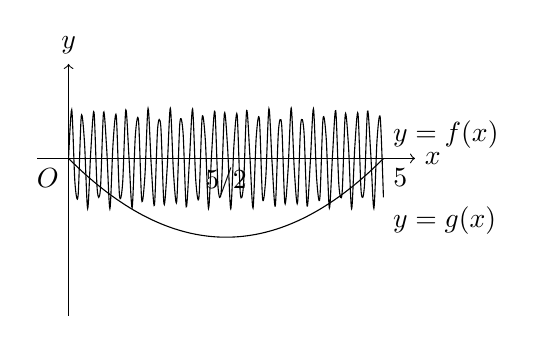
\begin{tikzpicture}[scale=0.8]
  \draw[->] (-0.5,0) -- (5.5,0) node[right] {$x$};
  \draw[->] (0,-2.5) -- (0,1.5) node[above] {$y$};
  \node[below left] at (0,0) {$O$};
  \draw[domain=0:5,samples=100,smooth] plot (\x, {0.2*(\x)^2 - \x}) node[above right] {$y=f(x)$};
  \draw[domain=0:5,samples=100,smooth] plot (\x, {0.8*sin(\x*180/5 r)}) node[below right] {$y=g(x)$};
  \node[below] at (2.5,0) {$5/2$};
  \node[below right] at (5,0) {$5$};
\end{tikzpicture}
\end{center}

\subsection*{第2問}

[解] $ABCD$ が一辺2の正方形であるとして良い。この時, $V-ABCD$ の高さは $1$ となる。 $(\because \text{題意})$
そこで, $A(1,1,0), B(1,-1,0), C(-1,-1,0), D(-1,1,0), V(0,0,1)$ なる空間座標をおく。対称性から面 $VAB$ と面 $VBC$ のなす角をしらべれば良い。
面 $VAB, VBC$ の法線ベクトル $\vec{n}, \vec{m}$ は
\[
\vec{n} = \begin{pmatrix} 1 \\ 0 \\ 1 \end{pmatrix}, \quad \vec{m} = \begin{pmatrix} 0 \\ -1 \\ 1 \end{pmatrix}
\]
である。これらのなす角を $\theta$ として,
\[
\cos\theta = \frac{\vec{n} \cdot \vec{m}}{|\vec{n}||\vec{m}|} = \frac{1}{\sqrt{2}\sqrt{2}} = \frac{1}{2}
\]
\[
\therefore \theta = \frac{\pi}{3} \quad (\because 0 \le \theta \le \pi)
\]
だから, 2面のなす角は $\frac{\pi}{3} \quad (<\pi/2)$ である。

\begin{center}
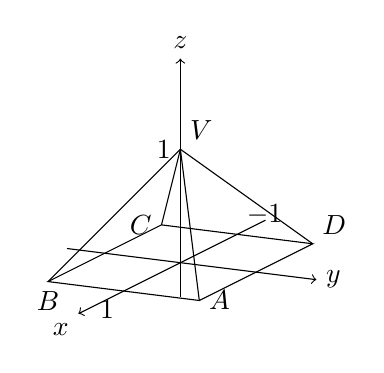
\begin{tikzpicture}[x={(-0.6cm,-0.3cm)}, y={(0.8cm,-0.1cm)}, z={(0cm,1.2cm)}, scale=1.2]
  \draw[->] (-1.5,0,0) -- (1.8,0,0) node[below left] {$x$};
  \draw[->] (0,-1.5,0) -- (0,1.8,0) node[right] {$y$};
  \draw[->] (0,0,-0.3) -- (0,0,1.8) node[above] {$z$};
  
  \coordinate (A) at (1,1,0);
  \coordinate (B) at (1,-1,0);
  \coordinate (C) at (-1,-1,0);
  \coordinate (D) at (-1,1,0);
  \coordinate (V) at (0,0,1);

  \draw (A) node[right] {$A$} -- (B) node[below] {$B$} -- (C) node[left] {$C$} -- (D) node[above right] {$D$} -- cycle;
  \draw (V) node[above right] {$V$} -- (A);
  \draw (V) -- (B);
  \draw (V) -- (C);
  \draw (V) -- (D);
  \node[left] at (0,0,1) {$1$};
  \node[below left] at (1,0,0) {$1$};
  \node[above right] at (-1,0,0) {$-1$};
\end{tikzpicture}
\end{center}

\subsection*{第3問}

[解] $a+b+c=0$ から,
\[
\begin{aligned}
f(x) &= ax^2 + bx - (a+b) \\
&= a(x^2-1) + b(x-1) \\
&= (x-1)\{a(x+1)+b\} \quad (a,b \in \mathbb{R}, a \neq 0) \quad \cdots \text{①}
\end{aligned}
\]
である。したがって, $\alpha, \beta$ が $1$ か否かで場合分けすれば良い。

$1^\circ$ $\alpha = \beta = 1$\\
①から, $f(\alpha) = f(\beta) = 0$ より, $(0,0)$ のみとる。

$2^\circ$ $\alpha = 1 \land \beta \neq 1$\\
$f(\alpha) = 0$, $f(\beta)$ は任意の生活をとるので, $X=0$

$3^\circ$ $\alpha \neq 1 \land \beta = 1$\\
$2^\circ$と同じく, $Y=0$

$4^\circ$ $\alpha \neq 1 \land \beta \neq 1$\\
この時, $(X,Y) = (f(\alpha), f(\beta))$ とすると
\[
\begin{pmatrix} X \\ Y \end{pmatrix} = a \begin{pmatrix} \alpha^2 - 1 \\ \beta^2 - 1 \end{pmatrix} + b \begin{pmatrix} \alpha - 1 \\ \beta - 1 \end{pmatrix}
\]
だから, まず第2文字 $b$ についてといて,
\[
b = \frac{1}{\alpha-1} X - (\alpha+1)a \quad (\because \alpha \neq 1)
\]
第1式に代入して,
\[
\begin{aligned}
Y &= (\beta^2-1) a + \frac{\beta-1}{\alpha-1} X - (\alpha+1)(\beta-1)a \\
&= \frac{\beta-1}{\alpha-1} X + (\beta-1)(\beta-\alpha) a
\end{aligned}
\]
ここでのち, $a \in \mathbb{R} \setminus \{0\}$ に注意して,
\begin{itemize}
  \item[ア] $\alpha \neq \beta$ の時, $Y \neq \frac{\beta-1}{\alpha-1} X$
  \item[イ] $\alpha = \beta$ の時, $Y = X$
\end{itemize
である。

以上まとめて,
\[
\begin{cases}
\alpha = \beta = 1 & \dots (0,0) \\
\alpha = 1 \land \beta \neq 1 & \dots X = 0 \\
\alpha \neq 1 \land \beta = 1 & \dots Y = 0 \\
\beta \neq \alpha \land \alpha \neq 1 \land \beta \neq 1 & \dots Y \neq \frac{\beta-1}{\alpha-1} X \text{ を満たす任意の点} \\
\beta = \alpha \land \alpha \neq 1 \land \beta \neq 1 & \dots Y = X
\end{cases}
\]

[解注]\\
$\begin{pmatrix} X \\ Y \end{pmatrix} = a \begin{pmatrix} \alpha^2-1 \\ \beta^2-1 \end{pmatrix} + b \begin{pmatrix} \alpha-1 \\ \beta-1 \end{pmatrix}$。ゆえ, $\begin{pmatrix} \alpha^2-1 \\ \beta^2-1 \end{pmatrix}, \begin{pmatrix} \alpha-1 \\ \beta-1 \end{pmatrix}$ が1次独立である条件をかんがえても ($\triangle$の面積が0でない) 良いか。

\subsection*{第4問}

[解] 平面 $z=k$ での切り口の面積 $S(k)$ は
\[
S(k) = \pi \{ 1 + (1-k^2)^2 \} = \pi \{ 2 - 2k^2 + k^4 \}
\]
だから, 求める体積 $V$ として
\[
\begin{aligned}
V &= \int_{-1}^1 S(k) \, dk \\
&= 2\pi \int_0^1 (2 - 2k^2 + k^4) \, dk \\
&= 2\pi \left[ 2k - \frac{2}{3}k^3 + \frac{1}{5}k^5 \right]_0^1 \\
&= \frac{46}{15}\pi
\end{aligned}
\]

\subsection*{第5問}

[解] (1) から $P(x)$ は奇関数で, $P(x) = ax^3 + bx \ (a \neq 0)$ とおける。\\
(2) から $b \neq 0$ である ($b=0$ なら $x=0$ が重根となり矛盾, 逆に $b \neq 0$ なら重根を作らない)。\\
さて, $P'(x) = 3ax^2 + b$ において, (3) から, $P'(x)$ が定符号である。\\
$ab \neq 0$ とあわせて,
\[
\begin{cases}
1^\circ \ a > 0 \land b > 0 \\
2^\circ \ a < 0 \land b < 0
\end{cases}
\]
のいずれかとなる。又, (4), (5) から
\[
\begin{cases}
P\left(\frac{1}{2}\right) = \frac{a}{8} + \frac{b}{2} \in \mathbb{Z} \quad \cdots \text{①} \\
0 < P(1) = a+b < 6 \quad \cdots \text{②}
\end{cases}
\]
$1^\circ$ 及び ②から, $2^\circ$ はありえず, $1^\circ$ に限定される。又, ①から
\[
\frac{a+4b}{8} \in \mathbb{Z} \quad \therefore a+4b = 8k \ (k \in \mathbb{N}) \quad \cdots \text{③}
\]
①,②から $(a,b) = (1,1),(1,2),(1,3),(1,4),(2,1),(2,2),(2,3),(3,1),(3,2),(4,1)$ となるが, ③を満たすのは $(a,b) = (4,1)$ のみ。したがって,
\[
P(x) = 4x^3 + x
\]

\subsection*{第6問}

[解] (1) $f(x) = (1+x)^\alpha - \left(1 + \frac{\alpha}{2} x\right)$ とおく。$f'(x) = \alpha \left[ \left(\frac{1}{1+x}\right)^{1-\alpha} - \frac{1}{2} \right]$ であり,\\
$0 \le x \le 1, 0 < \alpha < 1$ から, $\frac{1}{1+x} \ge \frac{1}{2}, 0 < 1-\alpha < 1$ であることより $f'(x) > 0$ だから $f(x)$ は単調増加で, $[0,1]$ の時, $f(x) \ge f(0) = 0 \quad \therefore 1 + \frac{\alpha}{2} x \le (1+x)^\alpha$

(2) $1 < \frac{1024}{1000} < 2^{\frac{1}{20}}$ $\dots$ ①を示す。①の左側は自明である。右側について, (1)で $(x, \alpha) = \left(1, \frac{1}{20}\right)$ とすると, (これは $0 \le x \le 1, 0 < \alpha < 1, \alpha \in \mathbb{Q}$ を満たす)
\[
2^{\frac{1}{20}} \ge 1 + \frac{1}{40} > 1 + \frac{24}{1000} \quad \left(\because \frac{1}{40} > \frac{24}{1000} \iff 1000 > 960\right)
\]
だから, ①の右側も成立。したがって①は成立する。①の両辺 1000 倍してから 20 乗すると,
\[
10^{60} < 2^{200} < 2 \cdot 10^{60} \quad \cdots \text{②}
\]
だから $2^{200}$ は, 61桁で, 最上位は 1.

(3) ②の各辺正だから常用対数をとって,
\[
60 < 200 \log_{10} 2 < 60 + \log_{10} 2
\]
\[
\therefore \frac{30}{100} < \log_{10} 2 < \frac{60}{199} \quad \cdots \text{③}
\]
となり,
\[
\frac{30}{100} = 0.300, \quad \frac{60}{199} = 0.3015 \dots < 0.302
\]
から,
\[
0.300 < \log_{10} 2 < 0.302
\]
となる。

\end{document}
